\section{Energy Modeling}
\label{sec:EnergyModeling}
Consider that the two seemingly best performing LPWAN technologies, LoRa and NB-IoT, are possible choices for our Elephant Tracking Application. We will now compare the energy consumption of these two technologies. 

As a constant, we will need to fix the Infrared Sensor that we will use in our application. For the purposes of this report, we will assume there is direct hardware compatability with the sensor and the LPWAN technology, and that we have done a control trial of using a smaller IR Sensor for detecting motion of the elephants at that specific range setting. 

The IR sensor we will be using is the \textit{GUMP's grocery HC-SR501 Infrared PIR Motion Sensor}\cite{GumpSensor}. This sensor has a range of 7 meters, and a power consumption of 60 $\mu$A, and since our operation will most likely be at the top end of its operational limit (farther to $7$ meters), we will assume that the device is operating at $20V$. Roughly speaking, we use this sensor as it is small and inconspicuous, and can be placed in the forest without being noticed by the elephants. That being said, the efficacy of the sensor is still in question, especially in a dense forest environment.\\
% \begin{figure}[!h]
    \centering
    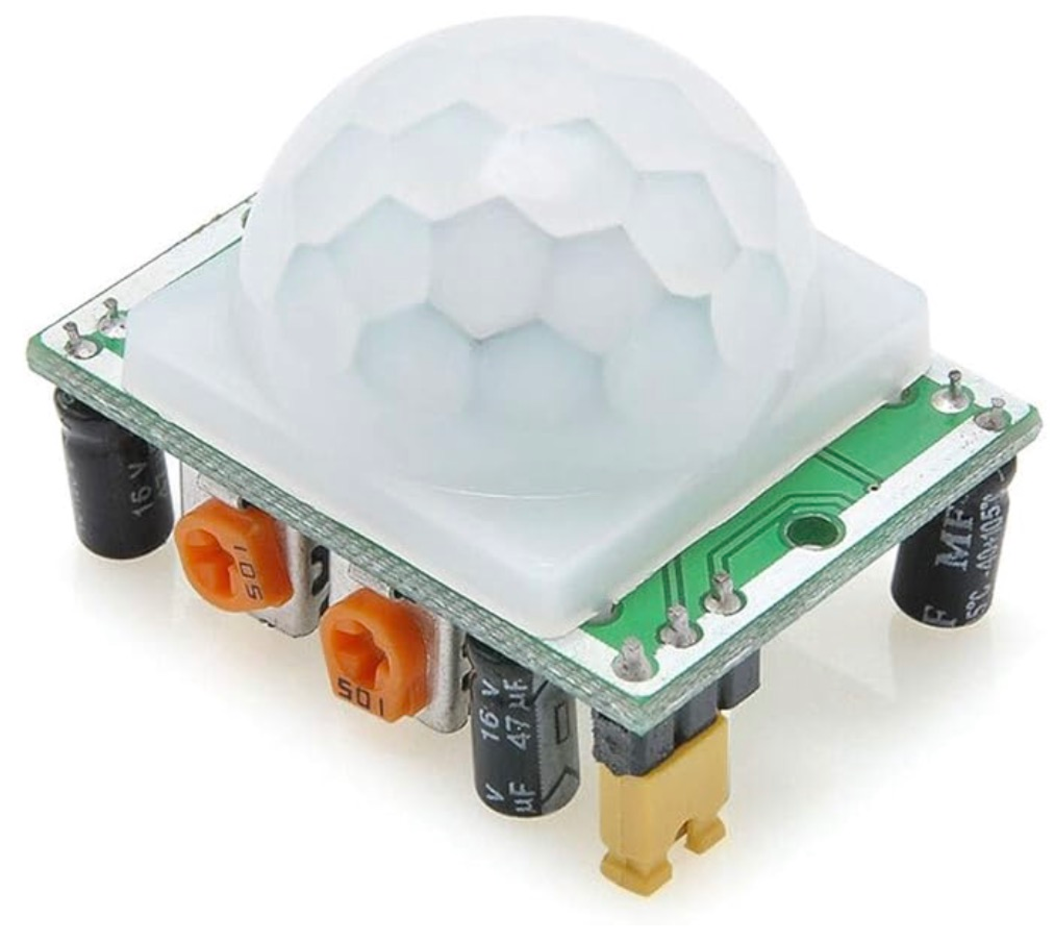
\includegraphics[width=0.6\columnwidth]{figures/Gump.pdf}
    \caption{GUMP HC-SR501 Infrared PIR Motion Sensor.}
    \label{fig:gump}
\end{figure}
\subsection{LoRa}
\label{sec:LoRa}
Our Application is based in Kerala $ + $ Tamil Nadu in India, so our LoRA specifications are different than the conventional US guidelines. In particular, in India we are able to use any Spreading Factor (SF) from SF7 to SF12, at 125 kHz bandwidth. This is because the Indian government has allocated the 865-867 MHz band for LoRaWAN use, which is different from the US guidelines. Another important thing is that according to \cite{loraGuidelines}, \textbf{there is no dwell or duty-cycle limitation on LoRA transmission}, according to Section 2.10.3 (IN865-867 Data Rate and End Device Output Power Encoding).


In the appendix, I've linked some of the LoRA quantities that are also found in screenshots (linked in appendix) from the Lora Guidelines. For our purposes, since we are using a Lora Module (I assume that we are using the SX1262 for transmit), and we will be comparing the power consumption of the device in both DC-DC and LDO mode. The LDO mode is more power hungry, and the DC-DC mode is more efficient. 

Consider the operating modes that we defined earlier: 
\begin{itemize}
    \item Steady State Sensing
    \item Event-Driven Update
    \item Emergency Mode
\end{itemize}
\subsubsection{Turning Off and On}
Since our time interval is so large, turning off the radio and then turning on will be marginal relative to the power consumption of the device. This is because either we will sleep for a long time, or we will be receiving for a long time, and the power consumption relative to the major operations of the device is in the order of nanoAmps versus Milliamps (nearly a factor of $10^6$). Susbequently, the datasheet provides the power consumption of the device in Sleep, but not necessarily the power consumption it takes to turn on the device $\rightarrow$ for the purposes of this report, we will assume that the power consumption of turning on the device is negligible (as a couple milliseconds relative to the 5 minute interval is not significant). 
In Steady State, the device will be in Sleep Mode for 5 minutes, wake up and second a transmission, and then go back to Sleep/standby. The power consumption for the Sleep duration is given by $1.2 \mu A \times 3.3 V * 300 s = 1.188 mJ$. This is with the crystal clock setting (XOSC) on. Then in Transmit this varies based on the power setting, let's see which mode is best for our application. 

Now the possible configurations we have for LoRA are 
$SF7, SF8, SF9, SF10, SF11, SF12$ at $125 kHz$ bandwidth. Then we can choose the power setting for the device, which can be $+14 dBm, +17 dBm, +20 dBm, +22 dBm$, as well as which mode we want to be in for hardware state (DC-DC or LDO).

For Steady State Sensing, we will sense for 1 second every 5 minutes, and then transmit accordingly based on our Spreading Factor prior to going back to standby. 

In general we have the formula $$E_{tx} = (\frac{P_{size}}{R} * I_{tx} * V_{opt}) * T_{tx} + E_{rest}$$, where $P_{size}$ is the packet size, $R$ is the data rate, and the other terms are the current, the operating Voltage, and the standby Energy. 

The Data rate will be dependent on the Spreading Factor, and the Current for Transmission will be dependent on the power setting.
\subsection{Steady State Transmission}
In essence, Table \ref{tab:lora_power_revised} contains simulated results of running the LoRa device under a Steady State configuration for 24 hours. The results are based on the power consumption of the device in different modes. Operating at SF7 with the lowest power setting of +14 dBm, the device consumes 30.310 J of energy over 24 hours, and this makes sense as the "chirps" are shorter and so messages can be transmitted faster. Intuitively, the higher the spreading factor, the more energy is consumed due to the longer chirps. At the highest end, SF12 with +22 dBm with a PA Target of +22 dBm, the device consumes 1.249 J of energy over 24 hours, nearly 30 times as much. This is a significant amount of energy, and it is clear that the device is not optimized for this setting. A configuration that strikes a sweet balance between energy consumption and data rate is SF7 with a +22 target with a Transmit Power of 22 dBm. This is the highest setting for the device, but by transmitting at a higher power, we still get a good data rate and a decent energy consumption of only 2.852 mJ over 24 hours, while still taking advantage of the LoRA's long range capabilities.

\subsection{Event-Driven Update}
In the cases where we do an update based on an event, ideally this is akin to a \textbf{Firmware Update} or a \textbf{Critical Event}. In this case, this is a downlink event where we will download a new patch, of 10 MB in size. Depending on our configuration, we can either use the DC-DC mode or the LDO mode. The DC-DC mode is more efficient, but the LDO mode is more power hungry.


It seems configuring the device to be in DC-DC mode is the best option for our firmware updates, as the power consumption is lower than in the LDO Mode. While we care about data integrity, the marginal optimization that LDO mode provides is not worth around 4 times the power consumption. Table \ref{tab:lora_rx} shows the power consumption of the device in the receive mode, and it is clear that the DC-DC mode is the best option for our application.

\subsection{Emergency Mode}

When the device is in Emergency Mode, we will be transmitting at the highest power setting, and we will be transmitting at the highest spreading factor. This is because we want to maximize the integrity of the device, and we want to ensure that the message is received. In this case, we will be transmitting at SF12, with a power setting of +22 dBm. This is the highest power setting for the device, and it is clear that the device is not optimized for this setting. The device consumes 1.638 J of energy over 24 hours, and this is a significant amount of energy. This is not a good setting for the device, and it is clear that the device is not optimized for this setting. We still aim to strike a good balance between power and data integrity, and we can still transmit at SF 12 with a +22 dBm power setting, but we will need to be more careful with our power consumption. A concern that is often brought up is that SF12 could cause an overlap in the chirps. This is a valid concern, but with our current packet structure of 16 bytes, we can still transmit at SF12 as the $TX$ duration is $\frac{16 * 8}{250} = 0.512 s$, which is less than the 10 second intermission between transmission.
\begin{figure*}[h!]
    \centering
    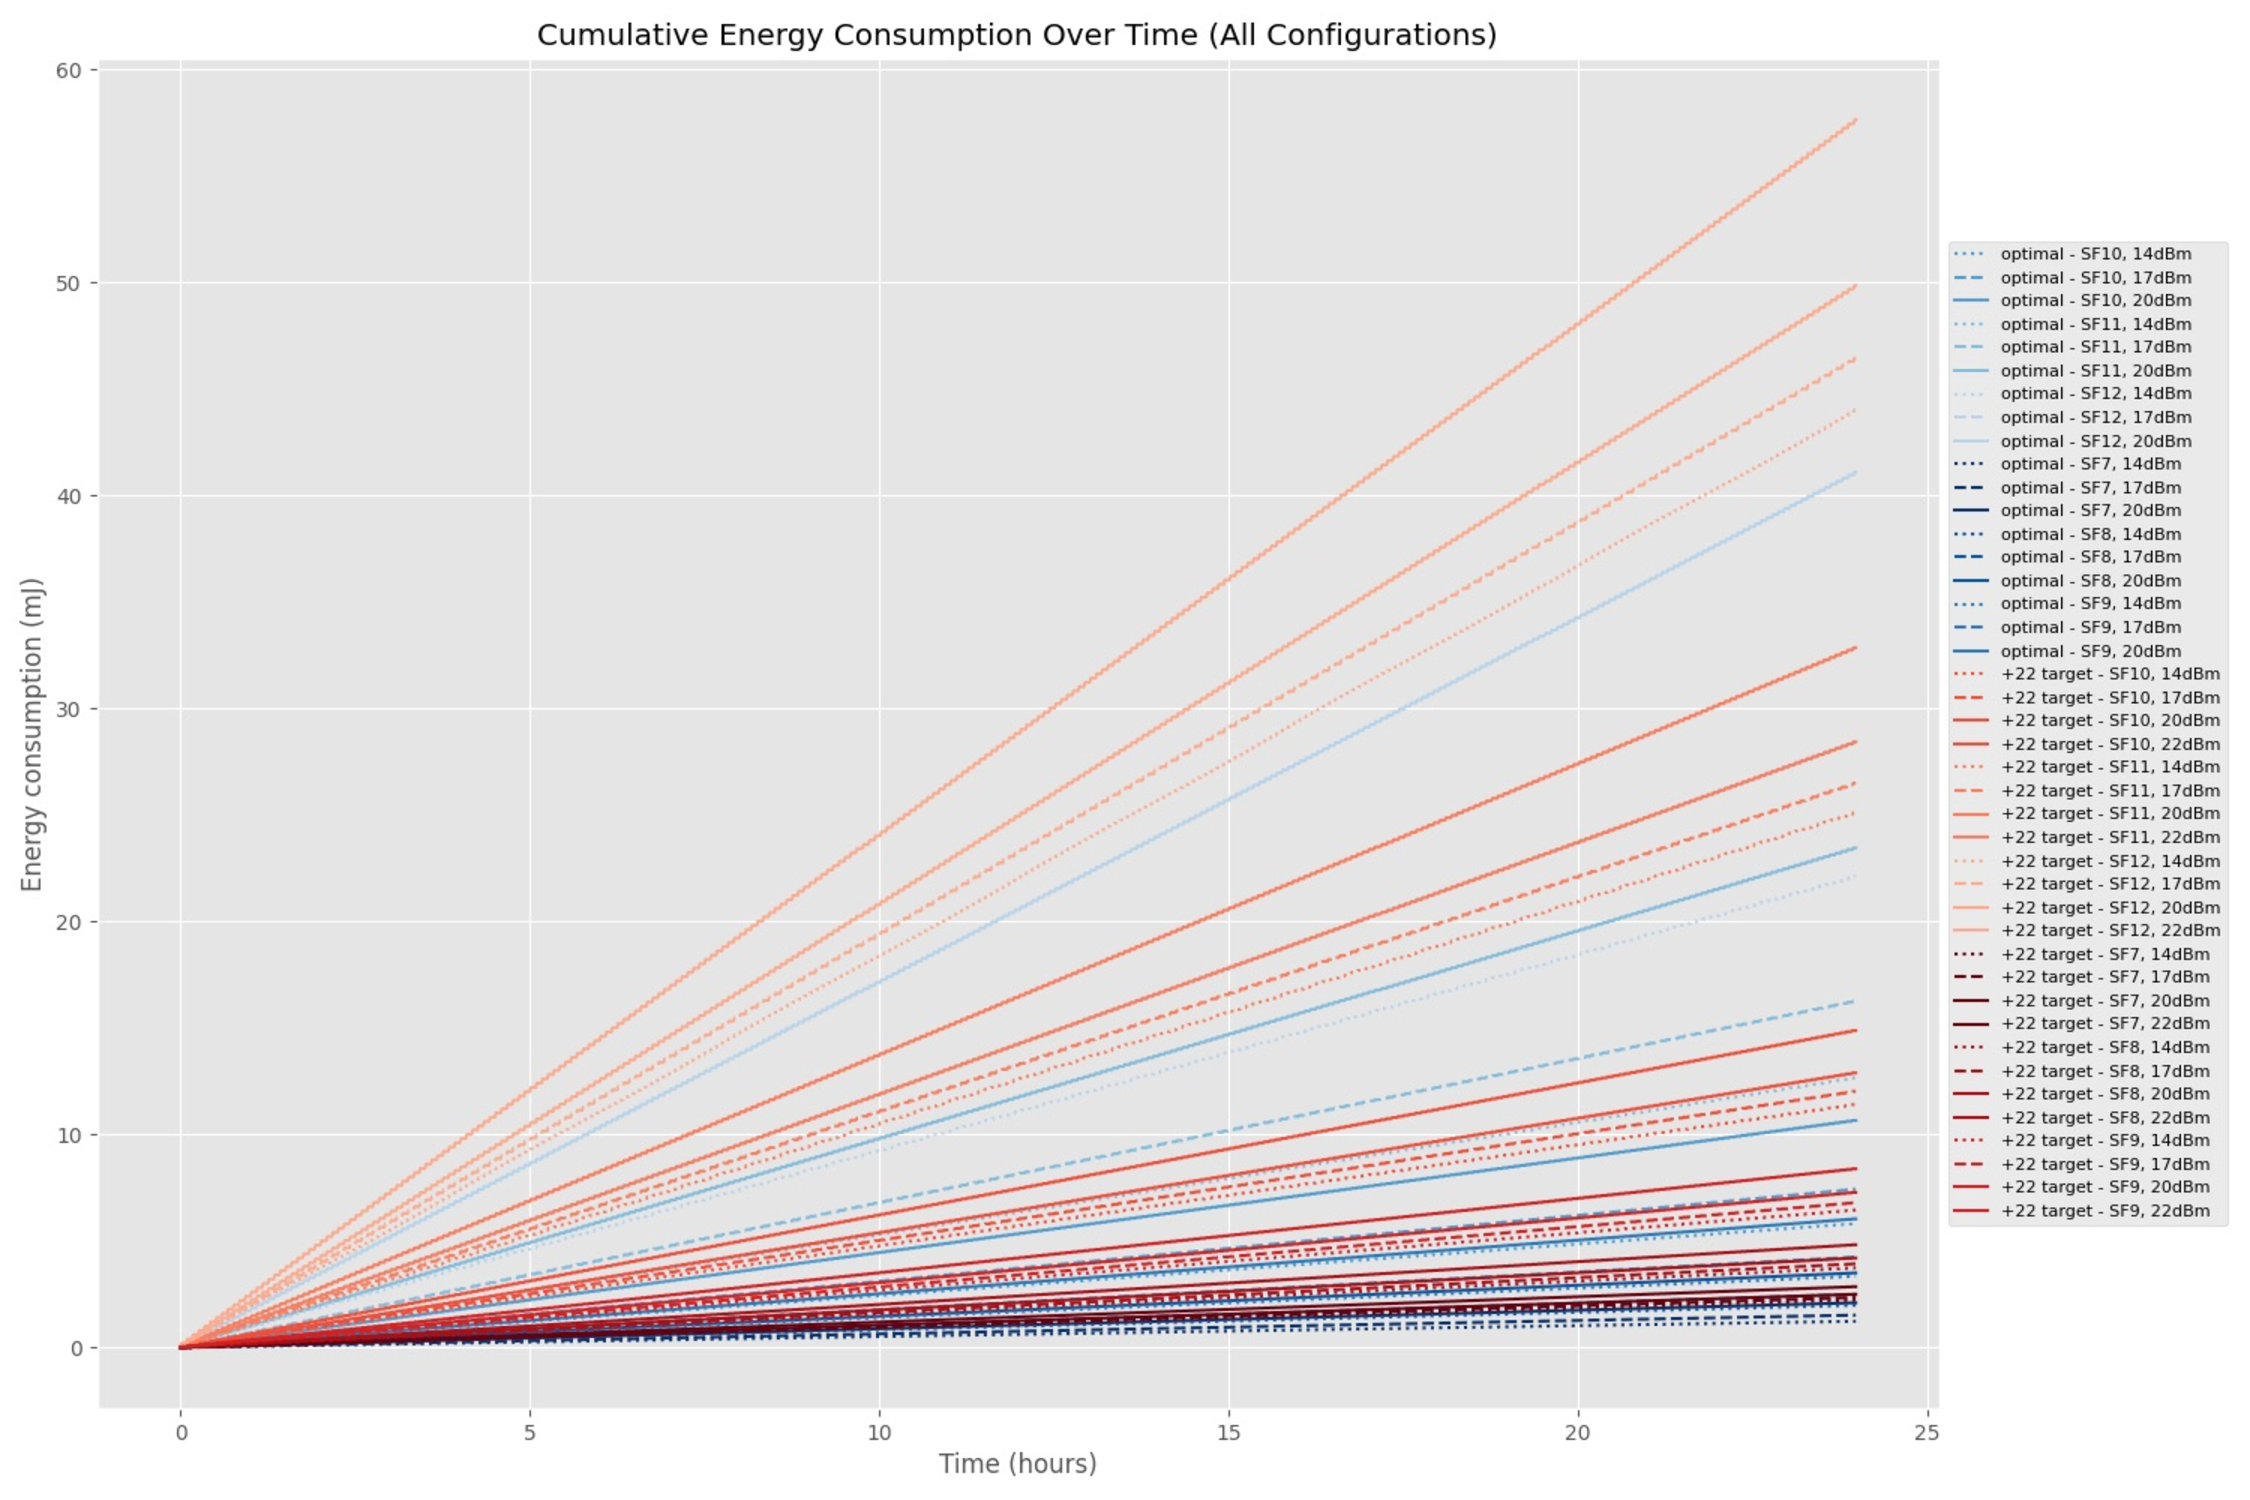
\includegraphics[width=\textwidth]{figures/loraTXSS.pdf}
    \caption{LoRa Device Power Consumption in Transmit Modes}
    \label{fig:loraTXSS}
\end{figure*}
\begin{figure}[h!]
    \centering
    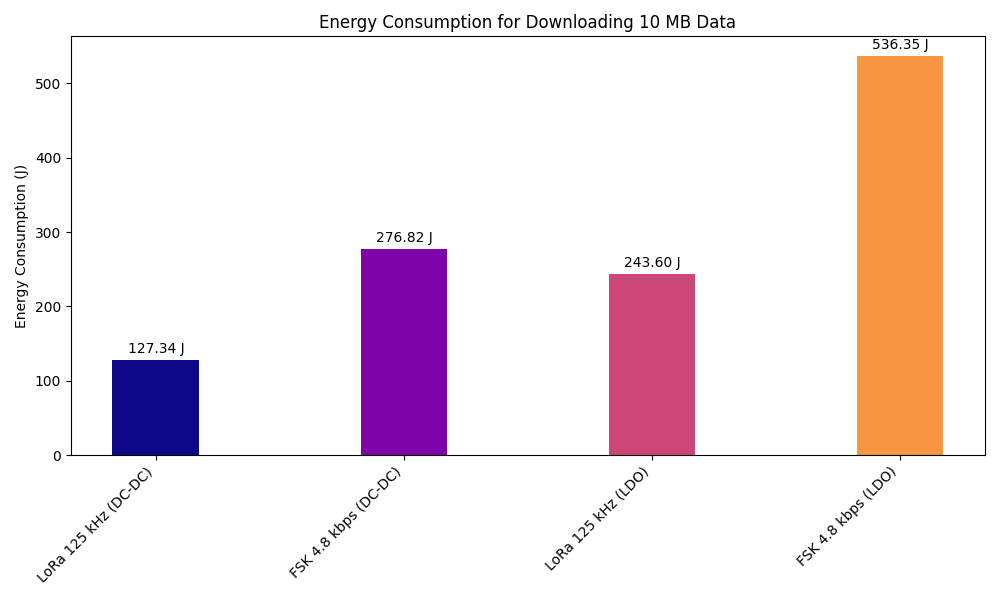
\includegraphics[width=\columnwidth]{figures/loraRx.png}
    \caption{LoRa Device Power Consumption in Receiving Firmware Update}
    \label{fig:loraRx}
    
\end{figure}
\begin{figure}[h!]
    \centering
    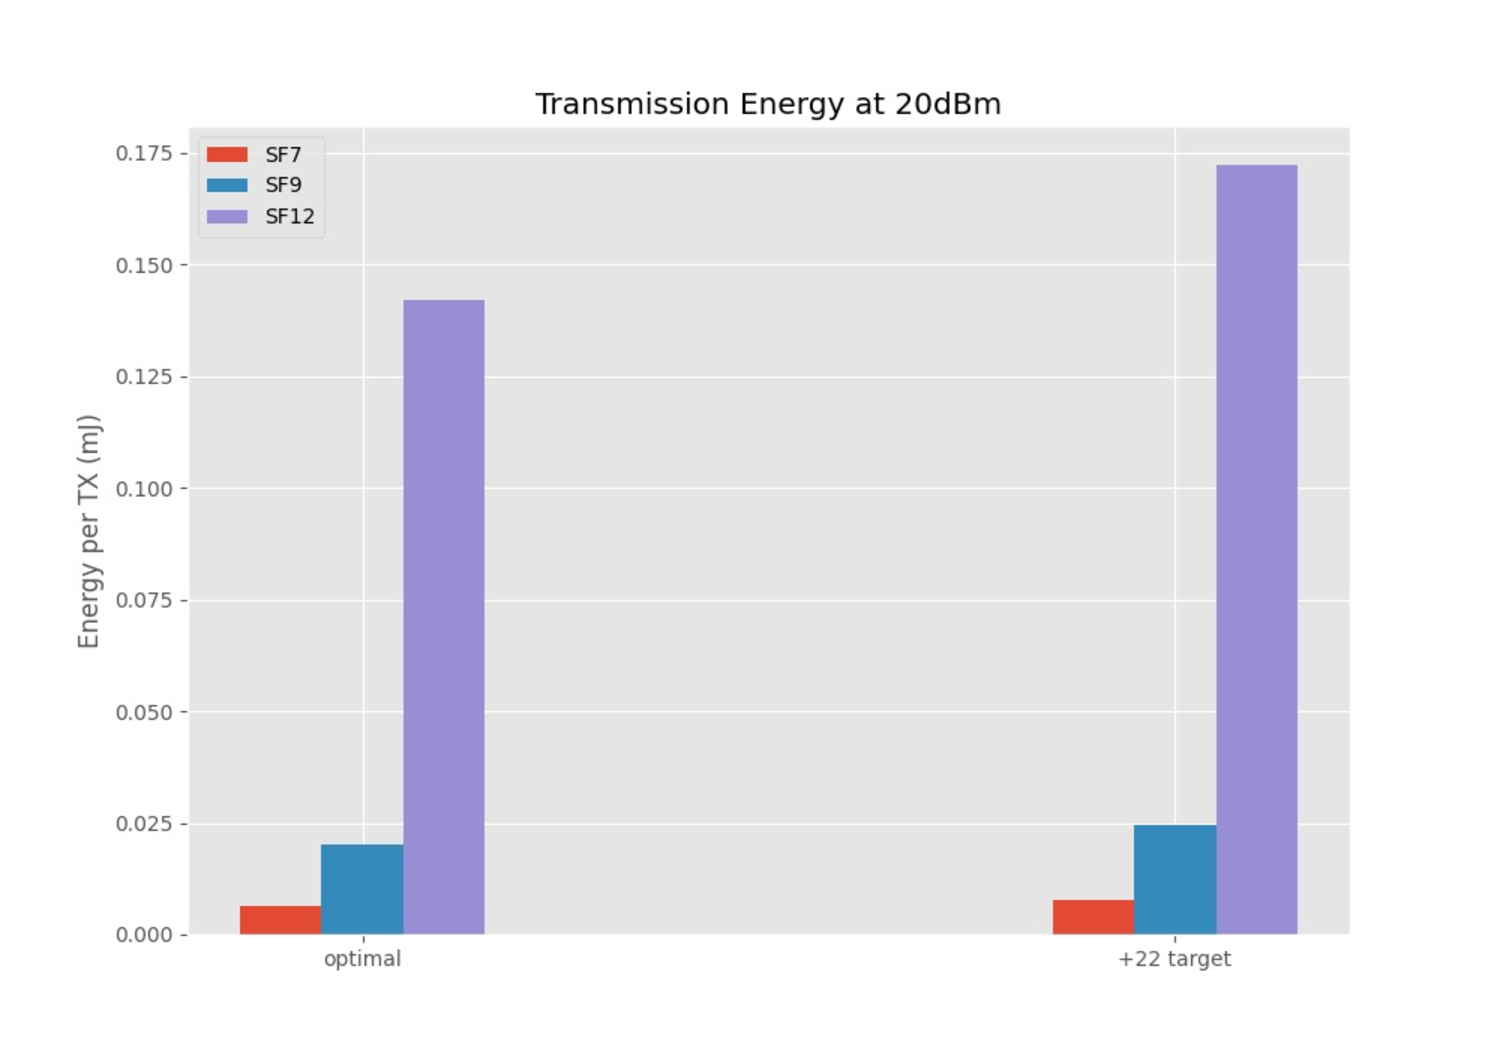
\includegraphics[width=\columnwidth]{figures/loratx20dbmbar.pdf}
    \caption{LoRa Device Power Consumption transmitting at +20 dBm}
    \label{fig:loratx20dbmbar}
\end{figure}

\subsection{NB-IoT}
\label{sec:NB-IoT}

Our Application can rely on the already existing 4G Infrastructure that already covers the entirety of continental India. That being said, power wise we don't have to deal with the complexities of changing a Spreading Factor Unlike LoRA, but we will have to tune some parameters to deal with our three different operating modes. 

The NB-IoT device will be in a similar configuration to the LoRA device, but the power consumption will be different. The device will be in Standby Mode for 5 minutes, wake up and send a transmission, and then go back to Standby/standby. The power consumption for this module is given by the same formula, but the current and voltage will be different. For brevity, \textbf{We will fix the module to the Sara R510S} for power consumption reasons (the initial deployment cost/cost of goods does not outweigh the module being performant for the entire year long pilot.)

Using the data sheet in \cite{nbPower}, there are many configurations for which we can configure the chip. Due to Discontinuous Reception (DRX), and Extended Discontinuous Reception (eDRX), we can model the power consumption of the device using different intervals. This plays to the strength of NB-IOT, where sleeping for a long time is beneficial, as this means less wake ups to sync with the central tower, and less power consumption overall. Also, while the device is operating, the typical operating voltage is $3.8V$ but this value ranges from $3.3 \sim 4.4$ V.

The main tradeoff with the NB-IOT approach is that while sleep mode is around the same as LORA, transmission is very high (around $2\sim3$ the magnitude to transfer at the same power strength as LoRA). But this is is a high level artifact of the technology, that can only be absorobed in our implementation due to current adoption standards of LoRA in India (and the ubiquitous nature of 4G and 5G in the region).

\subsection{Sleeping and Waking Up}
The datasheet specified that Power Off takes 0.5 $\mu A$ of current, but makes no mention of the power consumption of turning on the device. As with LoRA to keep a standardized metric across both wireless services, we will assume that the power consumption of turning on the device is negligible. This is because the use case of our application are such that the device will either be in standby for a long time (much larger than the time it takes to turn on the device), or the device will be transmitting for a long time (i.e. in Emergency Mode), or the device will be in a low power mode for a long time (i.e. in Steady State Sensing). Thus, the power consumption of turning on the device is negligible relative to the power consumption of the device in the major operations, especially when TX and RX are on the order of MilliAmps, and the difference from $0.5 \mu A$ to a TX state is around $1000 times$ the power consumption (i.e. we would need to turn on many times to make the power consumption of turning on the device significant).

\subsection{Steady State Sensing}
As with LoRA, the formula we have still holds where $$E_{tx} = (\frac{P_{size}}{R} * I_{tx} * V_{opt}) * T_{tx} + E_{rest}$$, where $P_{size}$ is the packet size, $R$ is the data rate, and the other terms are the current, the operating Voltage, and the standby Energy. Using the narrowband standard $NB-02$ which is the standard for this SARA R500S product line(and since we are using NB-IOT to maximize range), our data rate is 140 kbps UL and 125 kbps DL. The current for transmission is dependent on the power setting, and the operating voltage is $3.8V$. Based on Figure \ref{fig:NbTable}, we can set an \textit{Extended Disconnected Reception} window of nearly 65536 ms, which yields to an operating current of $1.1 mA$. Thus, while either in standby we will have $1.1 mA * 3.8 V * 300s = 1.089 J$ OR while off we'll have $0.5 \mu A * 3.8 V * 300s = 1.254 mJ$. This is roughly the same as LoRA for Switching off the device, but the power while sleeping is quite a bit higher (1.5x). 

What's key to understand though, is since the data rate is so high, the transmission time is much lower than LoRA, and the power consumption is much lower due to this. Consider the $T_{tx}$ for a LoRA with SF12, $\frac{16 * 8}{250} = 0.512 s$, but for NB-IOT, $\frac{16 * 8}{140000} = 0.1 ms$. This is a signifcant difference and so even if the power consumption is higher, the Power it takes for the device to transmit is much lower due to the high data rate. \textbf{This observation holds for even larger packet sizes}, because as we increase $|P_{tx}|$, the duration for both LoRA and NB-IOT increases linearly, but the duration for NB-IOT is still much lower than LoRA.

This is where $NB-IOT$ has a leg up quantitatively on LoRA, as in spite of having higher power consumption for TX, the \textbf{Interval transpired for the device to transmit is much lower}. This is a key point to consider, as the device will be transmitting for a much shorter time, and thus the power consumption is much lower.


\subsection{Event-Driven Update}
In the cases where we do an update based on an event, ideally this is akin to a \textbf{Firmware Update} or a \textbf{Critical Event}. When we listen for a 10 MB update from the tower, let's assume that the tower is transmitting at $+23 dBm$, then our RX current is now $195 mA$, much higher than the LoRA's 10.1 mA when listening at 125 kHz Bandwidth. This is a significant difference, and it is clear that NB-IOT is not optimized for listening or frequent TX/RX Transfer. To listen in for our firmware Update once a month, this is roughly the same as LoRA, where it's on the order of a couple hundred Joules. 

\subsection{Emergency Mode}
When the device is in Emergency Mode, we will be transmitting at the highest power setting, at +23 dBm. Based on our data so far, at this power setting, we use $395 mA$ of energy per transmission, but since we're still transmitting at the same data rate, the transmission time is still much lower than LoRA. Roughly, at $395 dBm$ when sleeping, we still only use $559.280 \mu J$ of energy, and this is much lower than LoRA. When standbying, we use $361.295 mJ$ of energy, which is still an order of magnitude less than LoRA. 


\section{Takeaways and Batteries}
\label{sec:Takeaways}
The optimal configuration for LoRA is to transmit at SF7 with a +22 dBm Power Setting, and this costs 78.662 mJ per day, and the optimal configuration for NB-IOT is to transmit at the highest power setting of +23 dBm, and this costs 559.280 $\mu J$ per day. This is a significant difference, and it is clear that NB-IOT is much more power efficient than LoRA. This is because the data rate for NB-IOT is much higher than LoRA, and the transmission time is much lower. This is a key point to consider, as the device will be transmitting for a much shorter time, and thus the power consumption is much lower. 

\section{Part C: Higher Level Findings + Batteries}
\section{Part C: Tradeoff Analysis and Final Assessment}
\subsection{Technology Comparison}
\begin{itemize}
    \item \textbf{NB-IoT:}
    \begin{itemize}
        \item \textit{Pros:} High reliability, quality-of-service (QoS) guarantees, integration with existing cellular networks, and extended coverage in rural areas.
        \item \textit{Cons:} Higher cost per data unit compared to LoRa; requires subscription-based pricing, though cellular homework shows competitive rates when scaled.
    \end{itemize}
    \item \textbf{LoRa:}
    \begin{itemize}
        \item \textit{Pros:} Extremely low power, lower hardware and deployment cost, and robust performance in low-data-rate scenarios.
        \item \textit{Cons:} Limited QoS guarantees, potential issues with scalability in dense deployments, and reliance on custom gateways.
    \end{itemize}
    \item \textbf{Why NB-IoT and LoRa?} 
    \begin{itemize}
        \item Our application requires low data rates (approximately 100 KB/day per node) and extended battery life.
        \item Both NB-IoT and LoRa excel in low-power operation and long-range connectivity. Cellular homework data indicates that emerging IoT cellular solutions (NB-IoT) are cost-effective for such use cases, while LoRa offers unparalleled power efficiency \cite{jio2022iot, telcel2022network}.
    \end{itemize}
\end{itemize}

\subsection{Deployment Strategy and Cost Analysis}
\begin{itemize}
    \item \textbf{Node Cost:} Approximately \$50 per node, scalable from a pilot of 100 to full deployments.
    \item \textbf{Operational Cost:} NB-IoT involves data subscription fees which, per cellular homework, are competitive when negotiated at scale (e.g., pilot cost estimation in India shows figures around \$20,000 for 1000 devices). LoRa deployments may avoid recurring fees with a privately managed gateway network.
    \item \textbf{Maintenance:} Low power design and potential solar augmentation minimize onsite maintenance visits.
\end{itemize}

\subsection{Final Assessment}
Given the low data workload, remote deployment conditions, and strict power/cost constraints, our design recommends:
\begin{itemize}
    \item \textbf{Primary Technology:} LoRa for its ultra-low power consumption and cost benefits. Best suited when budget and energy efficiency are paramount.
    \item \textbf{Secondary Option:} NB-IoT as a fallback or for applications where integration with existing cellular networks and better QoS is required.
    \item \textbf{Network Deployment:} A mesh network with strategically placed gateways ensuring robust coverage over the tracking area.
    \item \textbf{Data Management:} Central hub receives data from nodes, performs aggregation, and issues alerts in near real-time.
    \item \textbf{Cost and Power:} Each node is designed to operate for at least one year on a single AA lithium battery; pilot and full-scale costs remain within competitive limits based on current cellular and IoT pricing structures.
\end{itemize}

%%%%%%%%%%%%%%%%%%%%%%%%%%%%%%%%%%%%%%%%%%%%%%
\section{Figures and Sample Code for Graphs}
Below is sample LaTeX code for including figures and generating a simple data throughput graph.

Ultimately where each technology shines is that for \textbf{receiving}, not at faster speeds but to conserve energy in general, \textbf{LoRA is the better choice.} This is because the power consumption of the device in receive mode is much lower than NB-IOT. However, for \textbf{transmitting}, \textbf{NB-IOT is the better choice.} This is because the power consumption of the device in transmit mode is much lower than LoRA. This is a key point to consider, as the device will be transmitting for a much shorter time, and thus the power consumption is much lower. That being said, the power consumption of the device in Sleep mode is slightly smaller for NB-IOT, but standby is a bit higher (0.8 to 1.1 mA). That being said for gateways and perhaps for nodes that might have to listen often, LoRA is the better choice. Arguably it comes down to the role of the device in our application, for nodes that frequently have to undergo patches or updates, LoRA will suit them better, as they can save more energy when listening to larger updates. 

However, since the main proprietary goal of our application is to simply transmit frequently updates and not listen, NB-IOT is the better choice. This is because the power consumption of the device in transmit mode is much lower than LoRA, due to the fact that our transmit frequency is significantly higher ($140 kbps$ vs $5.47 kbps$). This is a key point to consider, as the device will be transmitting for a much shorter time, and thus the power consumption is much lower. That being said, if our NB-IOT service does not support such high speeds, metrics will lean more and more towards LoRA. 


\subsection{Battery}
\label{sec:Battery}

Consider a year long usage of the following application. This is modeled by the equation $E_{total} = E_{tx} + E_{rx} + E_{sleep}$, where $E_{tx}$ is the energy consumed by the device in transmit mode, $E_{rx}$ is the energy consumed by the device in receive mode, and $E_{sleep}$ is the energy consumed by the device in sleep mode.

Every month, we do an $E_{rx}$ for 10 MB, and then every 5 minutes, we send an update in Steady State sensing. For brevity, we generalize a trend in our network, s.t. \textbf{5\% of our time we are in Emergency Mode, and the other 95\% of the time in TX we are in Steady State Sensing}. This is a rough estimate, but it is a good approximation for our application. Intuitively, the search space is quite vast, and it's not practical to assume that more than $5\%$ of the time we will be in Emergency Mode (that means there will be a rampant Emergency Threat for nearly 19 days under this model).


Thus, the total energy consumed by the device in a year is given by $$E_{total} = 12 * E_{rx} + 12 * 24 * 30 * (0.95 * E_{steady} + 0.05 * E_{emerg})$$ . This is a rough estimate, but it is a good approximation for our application. It captures the essence of our end node behavior, that we will be updating once every month, and then transmitting every 5 minutes, and steady and emergency mode dictate how much we sleep and how often we transmit. 


Thus, the total energy for LoRA is
$$\begin{aligned}E_{year} = 12 * 243.605 J +&\\ 12 * 24 * 30 * (0.95 * 56.046 mJ + 0.05 * 1.638 J) \\&= 4090.91 J\end{aligned}$$

And the total energy for NB-IOT is
$$\begin{aligned}E_{year} = 12 * 497.28 J +&\\ 12 * 24 * 30 * (0.95 * 361.295 mJ + 0.05 * 559.280 \mu J) = 6.5 J \\&= 9174.478 J\end{aligned}$$

This is a significant difference, and it is clear that NB-IOT is much more power hungry than LoRA, that being said, existing infrastructure lends itself to a more optimal usage of NB-IOT, and the power consumption of the device in transmit mode is much lower than LoRA. Much of the change can also be chalked up to the fact that we chose a very unreliable medium of communication, choosing $SF7$, and $+20 dBm$ in contrast to overthrottling the NB-IOT device to transmit at its max $+23dBm$ with the max power setting. While it may seem that the power consumption of the device in transmit mode is much higher than LoRA, balancing data integrity for only 2 times the power is a good tradeoff that I am willing to balance. 


As such, a battery than can empirically support our system for a year must be a battery with at least $\frac{9175}{V_{nom}}$ mAh. Thus, we have two options: 
\begin{itemize}
    \item A Single 1.5 V D-Cell Battery with a capacity of around 15K mAh, some batteries are rated for $15K \sim 20K$ mAh, and this is a good choice for our application. This will last us for at least a year. At the standard $1.5V$ this is at least $22K mAh$, which could serve our end nodes for at least 2 years.\cite{Dcell}
    \item 3 AA Batteries in Series, with a capacity close to $2500 mAh$ each, $7500 * 1.5 V = 11250 mAh$, which is a bit lower than the D-Cell, but still a good choice for our application. This will last us for at least a year.\cite{AA}
\end{itemize}




